\documentclass{article}
\usepackage{amsmath}
\usepackage{amssymb}
\usepackage{tikz}
\usepackage{pgfplots}
\pgfplotsset{compat=1.18}
\usetikzlibrary{plotmarks}

\begin{document}

    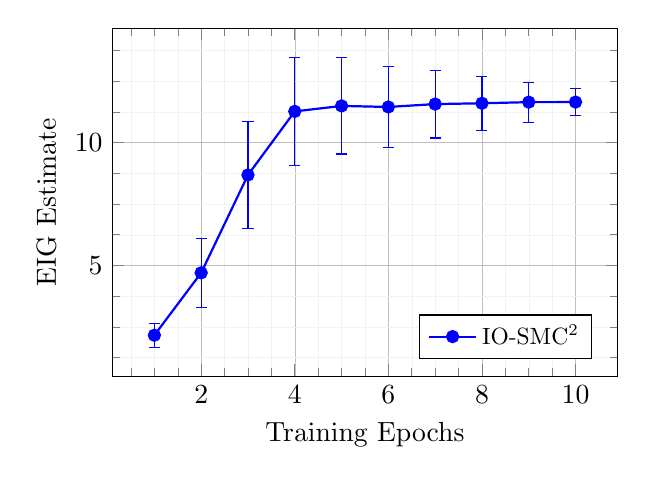
\begin{tikzpicture}

\begin{axis}[
    width=8cm,
    height=6cm,
    grid=both,
    minor tick num=3,
    grid style={line width=.1pt, draw=gray!10},
    major grid style={line width=.1pt, draw=gray!50},
    xlabel=Training Epochs,
    ylabel=EIG Estimate,
    legend style={
        nodes={scale=0.85, transform shape},
        at={(0.95,0.05)},
        anchor=south east
    },
    legend cell align={left},
]
    \addplot [
        blue,
        thick,
        mark=*,
        mark size=2,
        error bars/.cd,
            y dir=both,y explicit,
    ] coordinates {
        (1.0, 2.1572626566391357) +- (0.0, 0.4852629281775711)
        (2.0, 4.697847636406411) +- (0.0, 1.3938436910513539)
        (3.0, 8.682347981714873) +- (0.0, 2.178400520176821)
        (4.0, 11.270263109648816) +- (0.0, 2.205614456533889)
        (5.0, 11.492795869102457) +- (0.0, 1.958797491129598)
        (6.0, 11.450597768825343) +- (0.0, 1.6568317104629253)
        (7.0, 11.567711980314135) +- (0.0, 1.3814769045961826)
        (8.0, 11.600554473015073) +- (0.0, 1.1001655046738537)
        (9.0, 11.646722164747013) +- (0.0, 0.8127851066191146)
        (10.0, 11.649341359536166) +- (0.0, 0.5387024536491489)
    };
    \addlegendentry{IO-SMC\textsuperscript{2}}
\end{axis}
\end{tikzpicture}

\end{document}